\documentclass{beamer}
\usepackage{tikz}

% Use a custom beamer theme
\usetheme{CambridgeUS}
\usecolortheme{default} % 默认主题基础
\setbeamercolor{structure}{fg=red} % 设置结构颜色为红色
\setbeamercolor{title}{fg=red}     % 标题颜色为红色
\setbeamercolor{item}{fg=red}      % 项目符号为红色
\usepackage{tcolorbox}
\usepackage{siunitx}
    \sisetup{per-mode=symbol}
\usepackage{amsmath} % 数学公式支持
\usepackage{amssymb} % 数学符号支持
\usepackage{graphicx}


% Custom title slide settings

\setbeamertemplate{title page}{
    \begin{center}
        \vspace{1cm}
        \includegraphics[width=0.55\textwidth]{English logo.png}\\[0.5cm] % Replace with your logo file
        \textbf{\Large\textcolor{red}{Solving 2D Steady-State Heat Conduction Problems Using PINNs}} \\[1cm]
        \textbf{\large Jiaxin Wang}\\[0.2cm]
        \footnotesize China-UK Low Carbon College \\ 
        Shanghai Jiao Tong University \\[0.5cm]
        \textbf\footnotesize{\today}\\[1cm]
    \end{center}
}

\setbeamertemplate{frametitle}{
    \vbox{
        \hbox{
            \begin{minipage}[t]{0.8\textwidth}
                \usebeamercolor[fg]{frametitle}
                \strut\insertframetitle\strut
            \end{minipage}
            \begin{minipage}[t]{0.2\textwidth}
                \raggedleft
                \includegraphics[height=0.8cm]{English logo.png} % 替换为您的 logo 文件路径
            \end{minipage}
        }
        \vskip1ex % 控制标题和正文的间距
    }
}


\begin{document}

% Title slide
\begin{frame}
    \titlepage
\end{frame}

\begin{frame}
    \frametitle{Contents}
    \tableofcontents
\end{frame}

% Slide 1: Overview
\section{Introduction}
\begin{frame}{Solved problem}
    \begin{columns}
        % 左侧列(图片)
        \begin{column}{0.5\textwidth}
            \centering
            \includegraphics[width=\textwidth]{1.pdf} % 替换为图片路径
            \caption{\footnotesize Figure 1: Schematic diagram of the geometry of the research object}
        \end{column}

        % 右侧列(文字)
        \begin{column}{0.5\textwidth}
            \begin{itemize}
                \item \textbf{Description:} Two-dimensional steady-state heat conduction problem (flat plate)
                \item \textbf{Parameters:}
                \begin{table}[!htbp]
                    \centering
                    \begin{tabular}{l  | l}
                        \hline
                        Name & Value \\
                        \hline
                        \texttt{L}  & \SI{1}{\meter}\\
                        \texttt{W} & \SI{1}{\meter}  \\
                        \texttt{k}  & \SI{10}{\watt\per\meter\per\kelvin} \\
                        \texttt{$T_1$}& \SI{30}{\celsius} \\
                        \texttt{$q''_s$}& \SI{2000}{\watt\per\meter\squared}  \\
                        \hline
                    \end{tabular}
                    \label{doc}
                \end{table}
            \end{itemize}
        \end{column}
    \end{columns}
\end{frame}


\begin{frame}{Benchmark--Based on analytical solution:}
\begin{itemize}
    \item Governing equation:
            \begin{equation}
                \frac{\partial^2 T}{\partial x^2} + \frac{\partial^2 T}{\partial y^2} = 0
            \end{equation}
    \item Boundary conditions:
        \[
        T(0, y) = T_1, \quad T(L, y) = T_1, \quad \left. -k \frac{\partial T}{\partial y} \right|_{y=W} = q_s''
        \]
        \[
        T(x, 0) = T_1
        \]
    \item The temperature field is given by:
    \begin{equation}
    T(x,y) = T_1 + \frac{q_s'' L}{k} \sum_{n=1}^\infty \frac{2(-1)^{n+1}+2}{n^2\pi^2 \cosh \left( \frac{n\pi W}{L} \right) }\sin \frac{n\pi x}{L}\sinh\frac{n\pi y}{L}
    \end{equation}
\end{itemize}

\end{frame}


% Slide 2: Methodology
\section{Methodology}
\begin{frame}{Methodology}
Conventional method - numerical solution (Finite Difference (FDM)): 
    \begin{itemize} 
    \item Governing equation:
    \begin{equation}
    \frac{\partial^2 T}{\partial x^2} \approx \frac{T_{m+1,n} - 2T_{m,n} + T_{m-1,n}}{\Delta x^2}, \quad
    \frac{\partial^2 T}{\partial y^2} \approx \frac{T_{m,n+1} - 2T_{m,n} + T_{m,n-1}}{\Delta y^2}.
    \end{equation}
    \item Internal node \( T_{m,n} \):\[
T_{m,n} = \frac{1}{4} \left( T_{m+1,n} + T_{m-1,n} + T_{m,n+1} + T_{m,n-1} \right).
\]
    \item Top boundary:
            \[
            T(x, W) = T(x, W - \Delta y) + \frac{q_s}{k} \Delta y.
            \]
            \[
                T_{i, Ny-1} = T_{i, Ny-2} + \frac{q_s}{k} \Delta y.
            \]

    \end{itemize}
\end{frame}

\begin{frame}{Methodology}
Deep Learning Method: PINNs: 
\begin{columns}
        % 左侧列(图片)
        \begin{column}{0.5\textwidth}
            \centering
            \includegraphics[width=\textwidth]{ngrk_a_1971251_f0001_oc.jpg} % 替换为图片路径
            \caption{\footnotesize Figure 2: Schematic architecture of PINN}
        \end{column}

        % 右侧列(文字)
        \begin{column}{0.5\textwidth}
            \begin{itemize}
                \item \textbf{Deep Learning Frameworks:} TensorFlow(Python 3.12.4)
                \item \textbf{Structure:}
                \begin{table}[!htbp]
                    \centering
                    \begin{tabular}{l  | l}
                        \hline
                        \small Item & \small Value \\
                        \hline
                        \texttt{\small Input layer}  & \small 2 \\
                        \texttt{\small Hidden layer} & \small 3  \\
                        \texttt{\small Output layer}  & \small 1 \\
                        \texttt{\small Number of neurons}& \small 128  \\
                        \texttt{\small Activation}& \small tanh \\
                        \hline
                    \end{tabular}
                    \label{doc}
                \end{table}
                \item \textbf{LOSS:} PDE+BC
                
            \end{itemize}
        \end{column}
    \end{columns}
\end{frame}


% Slide 3: Results
\section{Results}
\begin{frame}{Preliminary results}
\begin{figure}[!htbp]
    \centering
    \includegraphics[width =0.8\textwidth]{weixin1_20241229231213.png}
    \label{SJTU}
\end{figure}
There are the following problems: 
\begin{itemize}
    \item There are differences between numerical solutions and analytical solutions
    \item Whether PINNs itself is trained accurately
\end{itemize}
\centering \textbf{So I started a series of checks and revisions}
\end{frame}



\begin{frame}{Numerical oscillation of analytical solutions (Gibbs phenomenon)}
When the number of accumulated terms (terms or Nterm) of the Fourier series is too large or the calculation point is close to the boundary, numerical oscillation may occur.
    \begin{columns}[c] % [c]表示垂直方向居中对齐
        % 左侧图片
        \begin{column}{0.5\textwidth}
            \centering
            \includegraphics[width=\textwidth]{tupian16.png} % 替换为左侧图片路径
            \caption{\footnotesize Figure 3: Single point calculation code snippet (before improvement)} % 左图标题
        \end{column}

        % 右侧图片
        \begin{column}{0.5\textwidth}
            \centering
            \includegraphics[width=\textwidth]{tupian17.png} % 替换为右侧图片路径
            \caption{\footnotesize Figure 4: Temperature matrix calculation code (improved)} % 右图标题
        \end{column}
    \end{columns}
\end{frame}



\begin{frame}{PINNs Improvements: Big LOSS}
\small Train LOSS: PDE LOSS+BC LOSS
\small \\Test LOSS: MSE of $T_{pred}$-$T_{exact}$(Analytical solution)
    \begin{columns}
        % 左侧列(图片)
        \begin{column}{0.5\textwidth}
            \centering
            \includegraphics[width=\textwidth]{tupian18.png} % 替换为图片路径
            \caption{Figure 5:Train and Test Loss Curves (Preliminary Results)}
        \end{column}

        % 右侧列(文字)
        \begin{column}{0.3\textwidth}
            \begin{table}[!htbp]
                \centering
                \begin{tabular}{l  | l}
                \hline
                    Epoch & Loss \\
                    \hline
                    \texttt{0}  & 42717.332 \\
                    \texttt{500} & 5751.163  \\
                    \texttt{1000}  & 374.523 \\
                    \texttt{1500}& 50.388 \\
                    \texttt{2000}& 18.233 \\
                    \texttt{2500}& 15.104 \\
                    \texttt{3000}& 16.012 \\
                    \texttt{3500}& 12.732 \\
                    \texttt{4000}& 10.645 \\
                    \texttt{4500}& 7.963 \\
                    \hline
                \end{tabular}
                \label{doc}
            \end{table}
        \end{column}
    \end{columns}
\end{frame}


\begin{frame}{PINNS Improvements}
Looking for reasons:

    \vspace{1em}
    \resizebox{\textwidth}{!}{
    \begin{table}[!htbp]
    \centering
    \begin{tabular}{l | l | l | l | l | l }
    \hline
        Epoch & Loss(PDE) & Loss(Left) & Loss(Right) & Loss(Bottom) & Loss(Top) \\
        \hline
        \texttt{0}    & \textbf{0.003} & 907  & 910  & 901  & \textbf{40083} \\
        \texttt{500}  & 659 & 1591 & 494  & 1076 & 2498  \\
        \texttt{1000} & 57  & 137  & 85   & 67   & 133    \\
        \texttt{1500} & 11  & 17   & 15   & 1    & 14      \\
        \texttt{2000} & 38  & 6    & 7    & 1    & 3        \\
        \texttt{...} & ...  & ...    & ...    & ...    & ... \\
        \hline
    \end{tabular}
    \label{loss_table}
\end{table}
}
\end{frame}

\begin{frame}{PINNs Improvements}
I tried the following methods: 
\begin{itemize}
    \item \textbf{Increasing data density (at the boundary 200 points change to 1000 points)}
    \item Changing the neural network structure
    \item Changing the activation function
    \item Normalization
\end{itemize}
\begin{table}[!htbp]
    \centering
    \begin{tabular}{l  | l}
    \hline
        Epoch & Loss \\
        \hline
        \texttt{0}  & 42720.121 \\
        \texttt{500} & 7403.849  \\
        \texttt{1000}  & 570.526 \\
        \texttt{...}& ... \\
        \hline
    \end{tabular}
    \label{doc}
\end{table}
\end{frame}


\begin{frame}{PINNs Improvements}
I tried the following methods: 
\begin{itemize}
    \item Increasing data density 
    \item \textbf{Changing the neural network structure}(From [2,128,128,128,1] to [2,128,128,128,128,1]
    \item Changing the activation function
    \item Normalization
\end{itemize}
\begin{table}[!htbp]
    \centering
    \begin{tabular}{l  | l}
    \hline
        Epoch & Loss \\
        \hline
        \texttt{0}  & 42720.121 \\
        \texttt{500} & 3495.059  \\
        \texttt{1000}  & 668.900 \\
        \texttt{...}& ... \\
        \hline
    \end{tabular}
    \label{doc}
\end{table}
\end{frame}


\begin{frame}{PINNs Improvements}
I tried the following methods: 
\begin{itemize}
    \item Increasing data density 
    \item \textbf{Changing the neural network structure}(From [2,128,128,128,1] to [2,64,128,256,128,1]
    \item Changing the activation function
    \item Normalization
\end{itemize}
\begin{table}[!htbp]
    \centering
    \begin{tabular}{l  | l}
    \hline
        Epoch & Loss \\
        \hline
        \texttt{0}  & 42717.351 \\
        \texttt{500} & 8737.0805  \\
        \texttt{1000}  & 1400.246 \\
        \texttt{...}& ... \\
        \hline
    \end{tabular}
    \label{doc}
\end{table}
\end{frame}


\begin{frame}{PINNs Improvements}
I tried the following methods: 
\begin{itemize}
    \item Increasing data density 
    \item Changing the neural network structure
    \item \textbf{Changing the activation function}(tanh change to ReLU)
    \item Normalization
\end{itemize}
\begin{table}[!htbp]
    \centering
    \begin{tabular}{l  | l}
    \hline
        Epoch & Loss \\
        \hline
        \texttt{0}  & 42691.0 \\
        \texttt{500} & 538.176  \\
        \texttt{1000}  & 4658.061 \\
        \texttt{1500}  & 17829.849 \\
        \texttt{...}& ... \\
        \hline
    \end{tabular}
    \label{doc}
\end{table}
\end{frame}

\begin{frame}{PINNs Improvements}
I tried the following methods: 
\begin{itemize}
    \item Increasing data density 
    \item Changing the neural network structure
    \item \textbf{Changing the activation function}(tanh change to Sigmoid)
    \item Normalization
\end{itemize}
\begin{table}[!htbp]
    \centering
    \begin{tabular}{l  | l}
    \hline
        Epoch & Loss \\
        \hline
        \texttt{0}  & 42832.625 \\
        \texttt{500} & 40003.890  \\
        \texttt{1000}  & 12709.675 \\
        \texttt{...}& ... \\
        \hline
    \end{tabular}
    \label{doc}
\end{table}
\end{frame}


\begin{frame}{PINNs Improvements}
I tried the following methods: 
\begin{itemize}
    \item Increasing data density (at the boundary)
    \item Changing the neural network structure
    \item Changing the activation function
    \item \textbf{Normalization}
    \begin{itemize}
        \item Define non-dimensional temperature:
            \begin{equation}
            \theta = \frac{T - T_i}{q_s'' L / k}
            \end{equation}
        \item Rewritten Governing equation(according to (1) and (2)):
            \begin{equation}
            \frac{\partial^2 \theta}{\partial x^2} + \frac{\partial^2 \theta}{\partial y^2} = 0
            \end{equation}
        \item Rewritten Boundary conditions(according to (2)):
            \[
            \theta(0, y) = 0, \quad \theta(L, y) = 0, \quad \theta(x, 0) = 0,\quad \left. \frac{\partial \theta}{\partial y} \right|_{y=W} = 1/L
            \]
    \end{itemize}
\end{itemize}
\end{frame}



\begin{frame}{PINNs Improvements}
Improvment:
    \begin{columns}
        % 左侧列(图片)
        \begin{column}{0.5\textwidth}
            \centering
            \includegraphics[width=\textwidth]{tupian19.png} % 替换为图片路径
        \end{column}

        % 右侧列(文字)
        \begin{column}{0.5\textwidth}
            \begin{table}[!htbp]
                \centering
                \begin{tabular}{l  | l | l}
                \hline
                    Epoch & Loss PDE & Loss BC \\
                    \hline
                    \texttt{0}  & 0.0007 & 0.8585 \\
                    \texttt{500} & 0.0013 & 0.0180 \\
                    \texttt{1000} & 0.0022 & 0.0149 \\
                    \texttt{1500} & 0.0017 & 0.0095 \\
                    \texttt{2000} & 0.0008 & 0.0070 \\
                    \texttt{2500} & 0.0006 & 0.0062 \\
                    \texttt{3000} & 0.0008 & 0.0067 \\
                    \texttt{3500} & 0.0005 & 0.0052 \\
                    \texttt{4000} & 0.0005 & 0.0044 \\
                    \texttt{4500} & 0.0005 & 0.0036 \\
                    \texttt{4900} & 0.0006 & 0.0038 \\
                    \hline
                \end{tabular}
                \label{doc}
            \end{table}
        \end{column}
    \end{columns}
\end{frame}


% Slide 4: Discussion and Conclusion
\section{Review}
\begin{frame}{About the results}
    \begin{figure}
        % 第一张图片(顶部)
        \includegraphics[width=0.7\textwidth]{tupian12.png} % 替换为图片路径
        \vspace{0.05cm} % 增加图片间距

        % 第二张图片(底部)
        \includegraphics[width=0.7\textwidth]{tupian15.png} % 替换为图片路径
    \end{figure}
\end{frame}

\begin{frame}{About the project}
    \begin{itemize}
        \item \textbf{Engineering Applications:} PINNs provides an efficient and accurate alternative for scenarios where analytical solutions are unavailable, or numerical computations are costly (e.g., complex boundary conditions, multi-physics coupling).
        \item \textbf{Research Potential:} With its efficiency and multi-physics problem-solving capability, PINNs can be further extended to other challenging problems (e.g., transient heat transfer, turbulence simulations).
    \end{itemize}
\end{frame}

\begin{frame}{About my Gains}
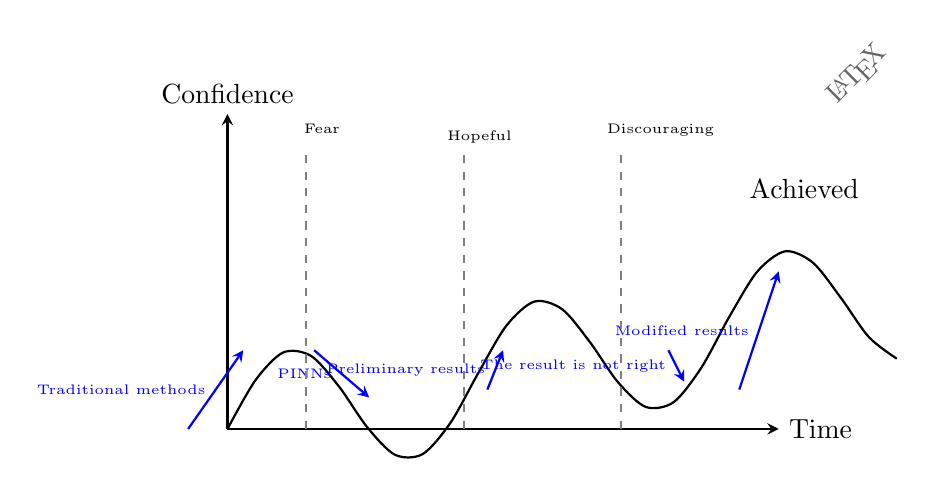
\begin{tikzpicture}[thick,>=stealth]

% 添加水印
\node[opacity=0.6, rotate=45, scale=1] at (8,4.5) {\LaTeX}; % 水印位置、透明度、大小

% 绘制坐标轴
\draw[->] (0,0) -- (7,0) node[right] {Time};       % 横轴,标注 "Time"
\draw[->] (0,0) -- (0,4) node[above] {Confidence}; % 纵轴,标注 "Confidence"

% 绘制主曲线
\draw[domain=0:8.5, smooth, variable=\r] plot ({\r}, {1.2*sin(2*\r r)*0.7 + 0.2*\r});

% 添加主要阶段标题
\node[below] at (1.2,4) {\tiny Fear};
\node[above] at (3.2,3.5) {\tiny Hopeful};
\node[below] at (5.5,4) {\tiny Discouraging};
\node[above right] at (6.5,2.8) {Achieved};

% 添加箭头和标注
\draw[blue,->] (-0.5,0) -- (0.2,1) node[midway, left] {\tiny Traditional methods};
\draw[blue,->] (1.1,1) -- (1.8,0.4) node[midway, left] {\tiny PINNs};
\draw[blue,->] (3.3,0.5) -- (3.5,1) node[midway, left] {\tiny Preliminary results};
\draw[blue,->] (5.6,1) -- (5.8,0.6) node[midway, left] {\tiny The result is not right};
\draw[blue,->] (6.5,0.5) -- (7,2) node[midway, left] {\tiny Modified results};

% 添加网格线(可选)
\draw[gray, dashed] (1,0) -- (1,3.5);
\draw[gray, dashed] (3,0) -- (3,3.5);
\draw[gray, dashed] (5,0) -- (5,3.5);

\end{tikzpicture}
\end{frame}


\end{document}


